\documentclass[border=6pt]{standalone}
\usepackage[T1]{fontenc}
\usepackage{tikz}
\usetikzlibrary{arrows.meta, positioning, decorations.pathreplacing, calc}

\definecolor{cInput}{RGB}{190,190,190}
\definecolor{cBlur}{RGB}{129,145,222}   % periwinkle blue
\definecolor{cSobel}{RGB}{96,181,171}   % teal
\definecolor{cNMS}{RGB}{235,165,64}     % orange
\definecolor{cHyst}{RGB}{219,101,101}   % red
\definecolor{cOutput}{RGB}{190,190,190}

\definecolor{cP1border}{RGB}{130,130,130} % Canny -- neutral grau

\definecolor{cP4fill}{RGB}{255,239,181}   % Song et al.        -- Gelb/Gold
\definecolor{cP4border}{RGB}{181,138,0}

\definecolor{cP2fill}{RGB}{250,214,231}   % Horvath et al.     -- Pink/Magenta
\definecolor{cP2border}{RGB}{188,42,110}

\definecolor{cP3fill}{RGB}{228,214,250}   % Ogawa et al.       -- Lila/Violett
\definecolor{cP3border}{RGB}{110,56,186}

\definecolor{cP5fill}{RGB}{240,222,201}   % Yadav & Gupta      -- Braun/Kupfer
\definecolor{cP5border}{RGB}{150,92,38}

\begin{document}
    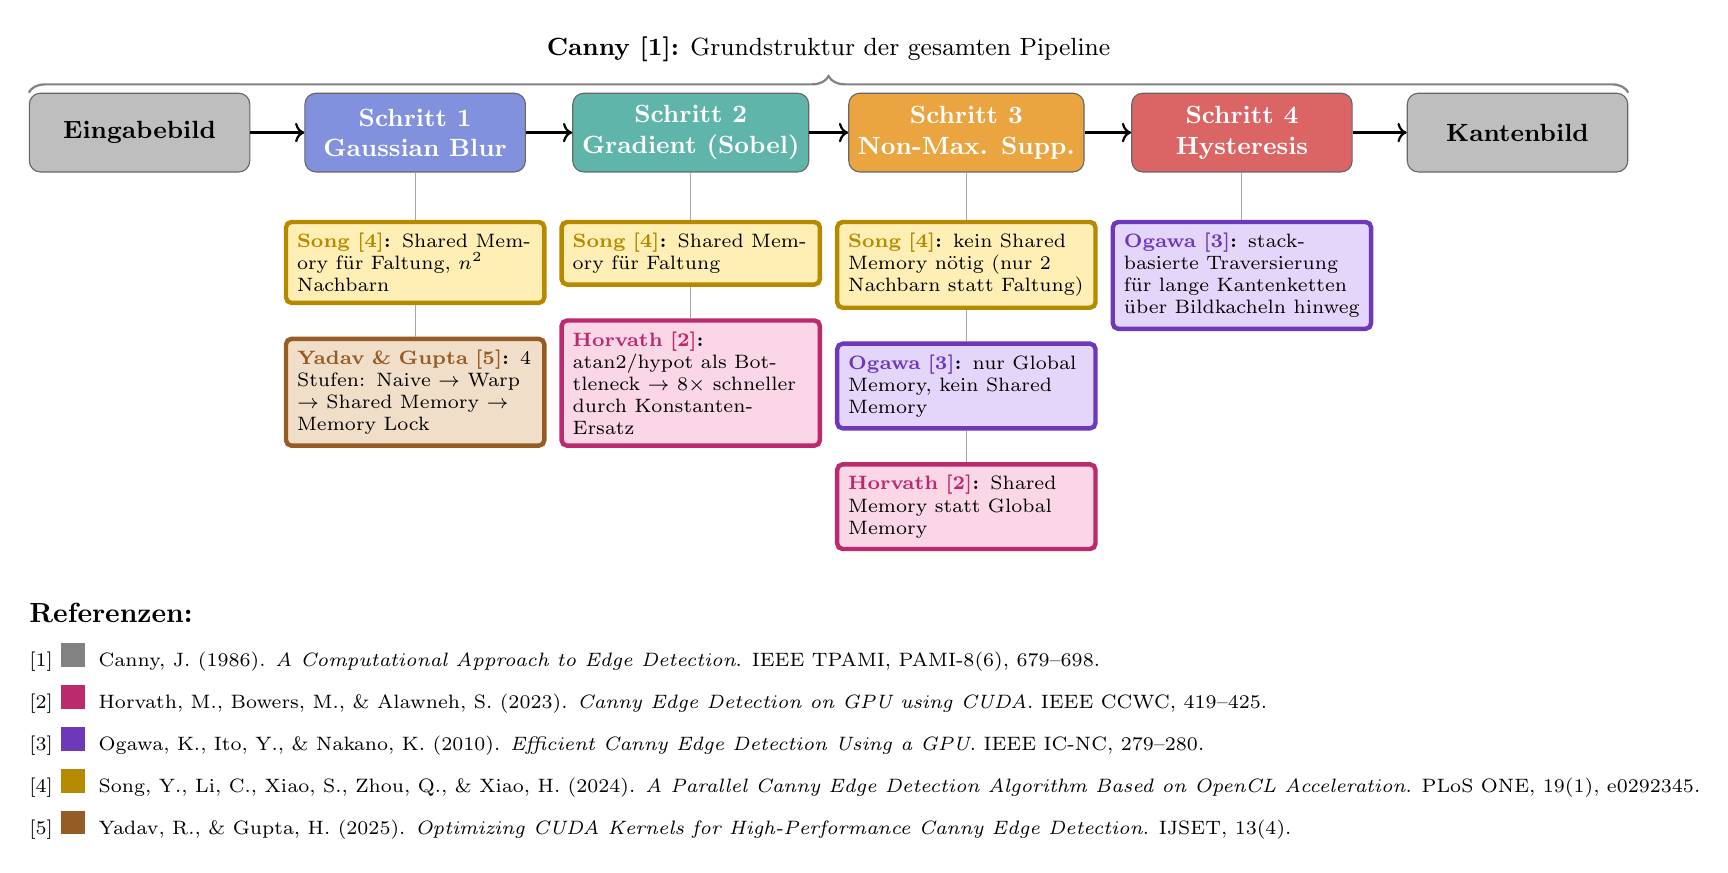
\begin{tikzpicture}[
        box/.style={rectangle, draw=black!60, rounded corners, minimum width=2.8cm,
        minimum height=1cm, align=center, font=\small\bfseries, text=white},
        annot/.style={rectangle, rounded corners=2pt,
        text width=3.0cm, align=left, font=\scriptsize, inner sep=4pt,
        line width=1.6pt},
        arrow/.style={->, thick},
        link/.style={gray!70, thin},
        legenditem/.style={font=\scriptsize, align=left, text width=15.8cm, inner sep=0pt}
    ]

        \node[box, fill=cInput, text=black]  (input)  at (0,0)    {Eingabebild};
        \node[box, fill=cBlur]   (blur)   at (3.5,0)  {Schritt 1\\Gaussian Blur};
        \node[box, fill=cSobel]  (sobel)  at (7,0)    {Schritt 2\\Gradient (Sobel)};
        \node[box, fill=cNMS]    (nms)    at (10.5,0) {Schritt 3\\Non-Max. Supp.};
        \node[box, fill=cHyst]   (hyst)   at (14,0)   {Schritt 4\\Hysteresis};
        \node[box, fill=cOutput, text=black] (output) at (17.5,0) {Kantenbild};

        \draw[arrow] (input)  -- (blur);
        \draw[arrow] (blur)   -- (sobel);
        \draw[arrow] (sobel)  -- (nms);
        \draw[arrow] (nms)    -- (hyst);
        \draw[arrow] (hyst)   -- (output);

        \draw[decorate, decoration={brace, amplitude=6pt}, thick, cP1border]
        (input.north west) -- (output.north east)
        node[midway, yshift=0.55cm, font=\small, text=black]
            {\textbf{Canny~[1]:} Grundstruktur der gesamten Pipeline};

        % --- Gaussian Blur ---
        \node[annot, fill=cP4fill, draw=cP4border, below=6mm of blur]  (blur1) {\textbf{\textcolor{cP4border}{Song~[4]}:} Shared Memory für Faltung, $n^2$ Nachbarn};
        \node[annot, fill=cP5fill, draw=cP5border, below=4mm of blur1] (blur2) {\textbf{\textcolor{cP5border}{Yadav \& Gupta~[5]}:} 4 Stufen: Naive $\rightarrow$ Warp $\rightarrow$ Shared Memory $\rightarrow$ Memory Lock};
        \draw[link] (blur.south) -- (blur1.north);
        \draw[link] (blur1.south) -- (blur2.north);

        % --- Sobel ---
        \node[annot, fill=cP4fill, draw=cP4border, below=6mm of sobel]  (sobel1) {\textbf{\textcolor{cP4border}{Song~[4]}:} Shared Memory für Faltung};
        \node[annot, fill=cP2fill, draw=cP2border, below=4mm of sobel1] (sobel2) {\textbf{\textcolor{cP2border}{Horvath~[2]}:} atan2/hypot als Bottleneck $\rightarrow$ 8$\times$ schneller durch Konstanten-Ersatz};
        \draw[link] (sobel.south) -- (sobel1.north);
        \draw[link] (sobel1.south) -- (sobel2.north);

        % --- NMS ---
        % Deliberate contrast between the three papers -- kept distinct,
        % not unified, since they genuinely differ:
        %   Song:    skips shared memory by design (only 2 neighbors, not a full conv.)
        %   Ogawa:   uses global memory only, no shared memory / tiling at all
        %   Horvath: does use shared-memory tiling for NMS
        \node[annot, fill=cP4fill, draw=cP4border, below=6mm of nms]  (nms1) {\textbf{\textcolor{cP4border}{Song~[4]}:} kein Shared Memory nötig (nur 2 Nachbarn statt Faltung)};
        \node[annot, fill=cP3fill, draw=cP3border, below=4mm of nms1] (nms2) {\textbf{\textcolor{cP3border}{Ogawa~[3]}:} nur Global Memory, kein Shared Memory};
        \node[annot, fill=cP2fill, draw=cP2border, below=4mm of nms2] (nms3) {\textbf{\textcolor{cP2border}{Horvath~[2]}:} Shared Memory statt Global Memory};
        \draw[link] (nms.south) -- (nms1.north);
        \draw[link] (nms1.south) -- (nms2.north);
        \draw[link] (nms2.south) -- (nms3.north);

        % --- Hysteresis ---
        \node[annot, fill=cP3fill, draw=cP3border, below=6mm of hyst] (hyst1) {\textbf{\textcolor{cP3border}{Ogawa~[3]}:} stack-basierte Traversierung für lange Kantenketten über Bildkacheln hinweg};
        \draw[link] (hyst.south) -- (hyst1.north);

        \node[anchor=north west, inner sep=0pt] (legend) at ($(input.west |- nms3.south) + (0,-6mm)$)
            {
            \begin{tabular}{@{}l@{\hspace{3pt}}c@{\hspace{5pt}}l@{}}
                \multicolumn{3}{@{}l@{}}{\normalsize\textbf{Referenzen:}} \\[4pt]
                \scriptsize [1] & \textcolor{cP1border}{\rule{0.3cm}{0.3cm}} & \scriptsize Canny, J. (1986). \textit{A Computational Approach to Edge Detection}. IEEE TPAMI, PAMI-8(6), 679--698. \\[3pt]
                \scriptsize [2] & \textcolor{cP2border}{\rule{0.3cm}{0.3cm}} & \scriptsize Horvath, M., Bowers, M., \& Alawneh, S. (2023). \textit{Canny Edge Detection on GPU using CUDA}. IEEE CCWC, 419--425. \\[3pt]
                \scriptsize [3] & \textcolor{cP3border}{\rule{0.3cm}{0.3cm}} & \scriptsize Ogawa, K., Ito, Y., \& Nakano, K. (2010). \textit{Efficient Canny Edge Detection Using a GPU}. IEEE IC-NC, 279--280. \\[3pt]
                \scriptsize [4] & \textcolor{cP4border}{\rule{0.3cm}{0.3cm}} & \scriptsize Song, Y., Li, C., Xiao, S., Zhou, Q., \& Xiao, H. (2024). \textit{A Parallel Canny Edge Detection Algorithm Based on OpenCL Acceleration}. PLoS ONE, 19(1), e0292345. \\[3pt]
                \scriptsize [5] & \textcolor{cP5border}{\rule{0.3cm}{0.3cm}} & \scriptsize Yadav, R., \& Gupta, H. (2025). \textit{Optimizing CUDA Kernels for High-Performance Canny Edge Detection}. IJSET, 13(4). \\
            \end{tabular}
        };

    \end{tikzpicture}
\end{document}